\section*{Химический состав растительной клетки}

\paragraph*{}Все химические вещества, входящие в состав клетки можно условно разделить на две группы:

\begin{enumerate}
	\item Конституционные -- служат для построения различных структур клетки
	\item Запасающие -- синтезируются как запас питательных веществ
\end{enumerate}

\paragraph*{}Массовая доля различных химических, входящих в состав клетки растения следующая:

\begin{itemize}

	\item 85\% вода
	\item 1,5\% другие неорганических веществ
	\item 10\% белки
	\item 1,1\% нуклеиновые кислоты
	\item 2\% липиды
	\item 0,4\% углеводы

\end{itemize}

\subsection*{Минеральные вещества} 

\subsubsection*{Вода}

\paragraph*{}В основном (80-90\%) \hyperlink{question_aqua}{воды} в клетке находится в особой органелле -- \hyperlink{question_vakual_rep}{центральной вакуоли}. 

\remember{Большая часть воды в клетке находится в \textbf{связанном} состоянии}

\paragraph*{}Различают следующие типы связанной воды:

\begin{enumerate}
	\item Осмотически-связанная низкомолекулярными соединений (моносахаридов, ионов и др.). Гидратирует ионы и коллоиды
	\item Коллоидно-связанная высокомолекулярными соединениями (целлюлоза, гемицеллюлоза, пектин, молекулы белка). Поддерживает структуру коллоидов и обеспечивает функционирование ферментов. Малоподвижна -- не участвует в растворении и транспорте веществ.
	\item Капиллярно-связанная -- в капиллярах клеточной стенки
	\item Химически связанная
\end{enumerate}

\paragraph*{}Роль воды в клетке растения:

\begin{enumerate}

   \item Участие в химических реакциях. Вода является средой где протекают химические реакции и непосредственным участником химических реакций. Например реакции фотосинтеза \ref{fotosynteses_example} идут в водной среде матрикса хлоропластов и при участии молекул воды.
   \item Поддержание структуры клеток. Форма клетки поддерживается за счет \termin{тургорного} давления воды. За счет высокого тургорного давления функционирует, например, механическая ткань \termin{колленхима} (\ris \ref{collenhima}).
   \item Транспорт веществ -- как органические так и неорганические вещества перемещаются внутри клетки и всего организма растения в растворенном виде.
   \item Участие в терморегуляции -- благодаря высокой теплоемкости вода способна смягчать воздействие на клетку резкого перепада температур.
   \item Участие в росте клетки -- клетка увеличивается в размерах за счет действия тургорного давления на клеточную стенку.

\end{enumerate}

\begin{equation}
	6H_{2}O + 6CO_{2} = C_{6}H_{12}O_{6} + 6O_{2}
	\label{fotosynteses_example}
\end{equation}

%%%%%%%%%%%%%%%%%%%%%%%%%%%%%%%%%%%%%%%%%%%%%%%%%%%%%%%%%%%%%%%%%%%%%%%%%%%%%%%%%%%%%%%%%%%%%%%%%%%%%%%%%%% 
\begin{figure}
  \centering
       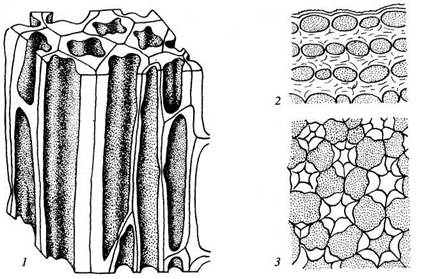
\includegraphics[width=0.5\linewidth]{pictures/collenhima}
\caption{Колленхима}
\label{collenhima}
\end{figure}
%%%%%%%%%%%%%%%%%%%%%%%%%%%%%%%%%%%%%%%%%%%%%%%%%%%%%%%%%%%%%%%%%%%%%%%%%%%%%%%%%%%%%%%%%%

\subsubsection*{Другие неорганические вещества}

\paragraph*{}Неорганические вещества, составляющие в клетке незначительную долю, представлены в основном ионами ($H^{+}$, $K^{+}$, $Na^{+}$, $Ca^{2+}$, $NH_{4}^{+}$ и анионами $OH^{-}$, $SO_{4}^{2+}$, $CO_{3}^{2-}$, $NO_{3}^{-}$, $Cl^{-}$). 

\paragraph*{}Часть от всего запаса неорганических ионов клетки всегда находится в вакуоли в растворенном состоянии и используется клеткой по мере необходимости. 

\paragraph*{}Функции ионов в клетке растения:

\begin{enumerate}
 \item Участие в биохимических процессах -- ионы могут являться элементами ферментов. 
 \item Создание электрического потенциала на мембране клетки
 \item Создание определенного осмотического давления. Осмос лежит в основе процессов поступления воды в растение и ее транспорта. Подробнее этот вопрос будет рассмотрен в разделе, посвященном \hyperlink{whater_circulation}{водному обмену}.
\end{enumerate}

%\paragraph*{}Основная роль ионов: участие в биохимических процессов в качестве составных элементов ферментов, неорганические ионы определяют электрический потенциал клетки участвуют в передаче импульсов возбуждения от клетки к клетке.

%\paragraph*{}Из неорганических веществ растительные клетки (а также, как известно из курса микробиологии, клетки микробов, ведущие фотосинтез и хемосинтез) способны синтезировать органические вещества, которые и определяют накопление биомассы в природы, являясь базовым звеном во всех биоценозах.

\subsection*{Органические вещества}

\paragraph*{}Органические вещества растительной клетки относятся к четырем основным группам\footnote{Так как особенности строения молекул и химические свойства органических веществ изучаются в курсе <<Органическая химия>>, то в данном разделе будет рассмотрена лишь роль различных органических веществ в клетке}

\begin{enumerate}

	\item углеводы
	\item липиды
	\item белки
	\item нуклеиновые кислоты

\end{enumerate}

\subsubsection*{Углеводы: строение, классификация и функции}.

\paragraph*{}\hypertarget{sect_glycosids}{Углеводы} или, сахара являются самыми распространенными в растении органическими веществами. Часть углеводов, например глюкоза, синтезируется в процессе фотосинтеза, другая часть синтезируется в ходе \gls{metabolism}а из других органических веществ. В дальнейшем, в процессе \gls{metabolism}а углеводы участвуют в создании различных органических веществ.

\paragraph*{}Углеводы делятся на 3 группы:

\begin{enumerate}

	\item моносахариды или монозы (простые сахара)
	\item олигосахариды
	\item полисахариды или полиозы

\end{enumerate}

\paragraph*{Моносахариды} -- простые молекулы с числом атомов углерода от 2 до 7. В соответствии с этим она называются: биозы, триозы, тетрозы, пентозы, гексозы, гептозы. Первые три - имеют линейную структуру молекул, последние - циклическую. Общая формула моноз 
$(CH_{2}O)_{n}$. Большинство углеводов в растительной клетке -- пентозы и гексозы.

\paragraph*{}Наиболее известные представители моноз - глюкоза, фруктоза и рибоза (\ris \ref{monogluc}). Монозы легко растворяются в воде, легко вступают в биохимические реакции. 

%%%%%%%%%%%%%%%%%%%%%%%%%%%%%%%%%%%%%%%%%%%%%%%%%%%%%%%%%%%%%%%%%%%%%%%%%%%%%%%%%%%%%%%%%%%%%%%%%%%%%%%

\begin{figure}[h]
\begin{minipage}[h]{0.3\linewidth}
\pyranose{5Sb==CH$_{2}$OH;1Sb==OH;1Sa==H;2Sb==H;2Sa==OH;3Sa==H;3Sb==OH;4Sb==H;4Sa==OH} \\ а) Глюкоза
\end{minipage}
\hfill
\begin{minipage}[h]{0.3\linewidth}
\furanose{4Sb==CH$_{2}$OH;4Sa==H;1Sa==CH$_{2}$OH;1Sb==OH;2Sa==H;2Sb==OH;3Sb==H;3Sa==OH} \\ б) Фруктоза
\end{minipage}
\begin{minipage}[h]{0.3\linewidth}
\furanose{4Sb==CH$_{2}$OH;4Sa==H;1Sa==H;1Sb==OH;2Sa==OH;2Sb==H;3Sb==H;3Sa==OH} \\ в) Рибоза
\end{minipage}
\caption{Моносахариды}
\label{monogluc}
\end{figure}

%%%%%%%%%%%%%%%%%%%%%%%%%%%%%%%%%%%%%%%%%%%%%%%%%%%%%%%%%%%%%%%%%%%%%%%%%%%%%%
\paragraph*{}Одни моносахариды в клетке легко превращаются в другие путем образования и распада фосфорных эфиров (\ris \ref{glucfos})

%%%%%%%%%%%%%%%%%%%%%%%%%%%%%%%%%%%%%%%%%%%%%%%%%%%%%%%%%%%%%%%%%%%%%%%%%%%%%%%%%%%%%%%%%%%%%%%%%%%%%%%%%%% 
\begin{figure}[h!]
  \centering
       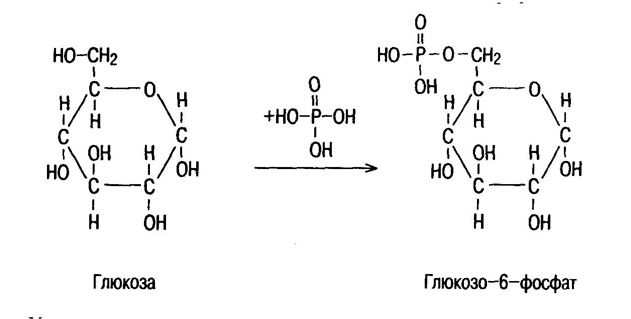
\includegraphics[width=0.5\linewidth]{pictures/glucfos}
\caption{Образование глюкозо фосфата}
\label{glucfos}
\end{figure}
%%%%%%%%%%%%%%%%%%%%%%%%%%%%%%%%%%%%%%%%%%%%%%%%%%%%%%%%%%%%%%%%%%%%%%%%%%%%%%%%%%%%%%%%%% 

\paragraph*{}Как вам известно из курса органической химии, моносахарам свойственна стереоскопическая \hyperlink{question_isomeria_gluc}{изомерия}. При этом в живых организмах сахариды представлены D-изомерами.

%%%%%%%%%%%%%%%%%%%%%%%%%%%%%%%%%%%%%%%%%%%%%%%%%%%%%%%%%%%%%%%%%%%%%%%%%%%%%%%%%%%%%%%%%%%%%%%%%%%%%%%%%%% 
\begin{figure}[h!]
  \centering
       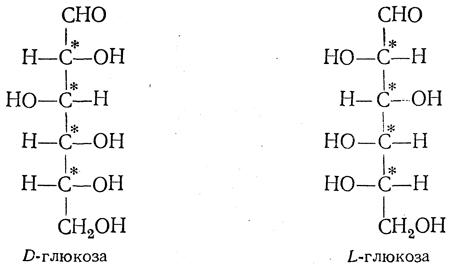
\includegraphics[width=0.5\linewidth]{pictures/dlgluk}
\caption{Моносахариды}
\label{monogluc}
\end{figure}
%%%%%%%%%%%%%%%%%%%%%%%%%%%%%%%%%%%%%%%%%%%%%%%%%%%%%%%%%%%%%%%%%%%%%%%%%%%%%%%%%%%%%%%%%% 

\paragraph*{}Функции моносахаридов:

\begin{enumerate}
	\item Метаболитическая -- глюкоза является субстратом для процессов дыхания и брожения. Глюкоза является исходным веществом для синтеза \hyperlink{krahmal}{крахмала} и \hyperlink{cellulosa}{целлюлозы}. Рибулеза участвует в синтезе углеводов в ходе фотосинтеза, являясь одним из звеньев цикла Кальвина
	\item Структурная -- Рибоза и дезокисрибоза входят в состав нуклеиновых кислот и \gls{atp}
	\item Запасающая -- Глюкоза и фруктоза выступают запасающими веществами в плодах
\end{enumerate}

\paragraph*{Олигосахара} -- это относительно простые молекулы, состоящие всего из 2-3 молекул моноз. В результате гидролиза олигосахаридов образуются моносахара (\ris \ref{hydrolis}).

%%%%%%%%%%%%%%%%%%%%%%%%%%%%%%%%%%%%%%%%%%%%%%%%%%%%%%%%%%%%%%%%%%%%%%%%%%%%%%%%%%%%%%%%%%%%%%%%%%%%%%%%%%% 
\begin{figure}[h!]
  \centering
       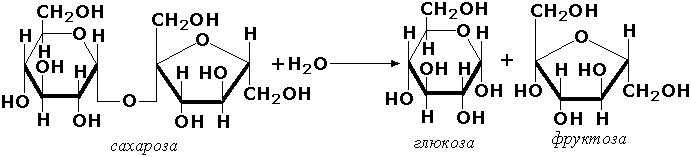
\includegraphics[width=0.5\linewidth]{pictures/hydrolis}
\caption{Гидролиз сахарозы}
\label{hydrolis}
\end{figure}
%%%%%%%%%%%%%%%%%%%%%%%%%%%%%%%%%%%%%%%%%%%%%%%%%%%%%%%%%%%%%%%%%%%%%%%%%%%%%%%%%%%%%%%%%%

\paragraph*{}Наиболее известный представитель олигосахаридов - сахароза. Олигосахариды легко растворяются в воде, участвуют в реакциях синтеза более сложных сахаров.

\paragraph*{}Функции олигосахаридов 

\begin{enumerate}
	\item Запасающая -- сахароза выступает запасающим веществом в корнеплодах свеклы, луковицах лука \cite{zauralov_1995}
	\item Транспортная -- углеводы перемещаются по организму растения в основном в виде сахарозы
\end{enumerate}

\paragraph*{Полисахариды} -- \termin{полимеры}, т.е. сложные молекулы, мономерами которых являются моносахара. Полисахариды нерастворимы в воде и обладают сложной структурой.

\paragraph*{}Наиболее известные представители полисахаридов: \hypertarget{krahmal}{крахмал}, гликоген, \hypertarget{cellulosa}{целлюлоза}, пектины.

\paragraph*{}Крахмал -- это полимер образованный $\alpha$-D глюкозой (\ris \ref{krahmal_mol}).  	

%%%%%%%%%%%%%%%%%%%%%%%%%%%%%%%%%%%%%%%%%%%%%%%%%%%%%%%%%%%%%%%%%%%%%%%%%%%%%%%%%%%%%%%%%%%%%%%%%%%%%%%%%%% 
\begin{figure}[h!]
  \centering
       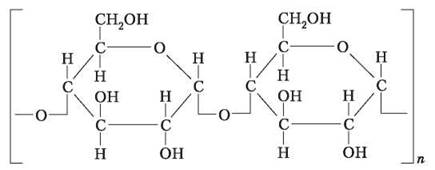
\includegraphics[width=0.5\linewidth]{pictures/krahmal_mol}
\caption{Структура молекулы крахмала}
\label{krahmal_mol}
\end{figure}
%%%%%%%%%%%%%%%%%%%%%%%%%%%%%%%%%%%%%%%%%%%%%%%%%%%%%%%%%%%%%%%%%%%%%%%%%%%%%%%%%%%%%%%%%%

\paragraph*{}Крахмал -- смесь двух гомополисахаридов: линейного -- \termin{амилозы} и разветвленного -- \termin{амилопектина}, общая формула которых $(С_{6}Н_{10}О_{5})_{n}$. Как правило, содержание амилозы в крахмале составляет 10–30\%, амилопектина – 70–90\%. Крахмал имеет молекулярную массу $10^{5}–10^{7}$ \gls{dalton}

\paragraph*{}При действии ферментов или нагревании с кислотами подвергается гидролизу. 

\paragraph*{}Целлюлоза -- это полимер образованный $\beta$-D глюкозой (\ris \ref{cell_mol}).

%%%%%%%%%%%%%%%%%%%%%%%%%%%%%%%%%%%%%%%%%%%%%%%%%%%%%%%%%%%%%%%%%%%%%%%%%%%%%%%%%%%%%%%%%%%%%%%%%%%%%%%%%%% 
\begin{figure}[h!]
  \centering
       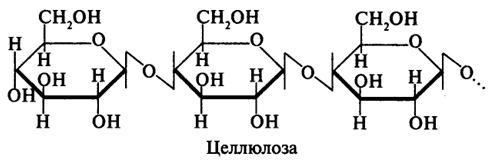
\includegraphics[width=0.5\linewidth]{pictures/cell_mol}
\caption{Структура молекулы целлюлозы}
\label{cell_mol}
\end{figure}
%%%%%%%%%%%%%%%%%%%%%%%%%%%%%%%%%%%%%%%%%%%%%%%%%%%%%%%%%%%%%%%%%%%%%%%%%%%%%%%%%%%%%%%%%%

\paragraph*{}При частичном гидролизе целлюлозы образуется дисахарид \termin{целлобиоза}, а при полном гидролизе – D-глюкоза. Молекулярная масса целлюлозы 1000–2000 кДа. 

\paragraph*{}Инулин – полисахарид, содержащийся в клубнях и корнях георгинов, артишоков и одуванчиков. При его гидролизе образуется фруктоза.

\paragraph*{}Функции Полисахаридов:

\begin{enumerate}

	\item Энергетическая -- при гидролизе полисахаридов образуется глюкоза или фруктоза которые затем могут использоваться растениями в ходе метаболизма.
	\item Строительная -- Целлюлоза и пектин входят в состав \hyperlink{cell_wall}{клеточной стенки}
	\item Запасающая -- крахмал является основным запасным питательным веществом в растении. Главным образом накапливается в семенах (зерна злаков содержат до 70\% крахмала), а также в луковицах, клубнях и сердцевине стебля растений (до 30\%). В небольших количествах он содержится в листьях.

\end{enumerate}

\remember{Крахмал является основным запасным питательным веществом в растении}

\subsubsection*{Липиды: строение, классификация и функции}

\paragraph*{}\hypertarget{sect_lipids}{Липиды} представляют собой достаточно сложные по химической структуре вещества. В их состав также входят углерод, кислород, водород, но в отдельные группы липидов могут входить фосфор, сера, и азот (фосфатиды, пигменты). Все липиды гидрофобны. Функции липидов различны в зависимости от химического строения. Липиды не являются биополимерами.

\remember{Так как жиры не растворимы в воде, они не способны передвигаться по растению. Жиры синтезируются в митохондриях и остаются там до момента использования}

\paragraph*{}Липиды классифицируются на 5 больших групп по признаку функции и сложности строения:

\begin{enumerate}

	\item Жиры
	\item Воска
	\item Фосфатиды
	\item Пигменты
	\item Стероиды
	
\end{enumerate}

\paragraph*{Жиры} или это эфиры состоящие из глицерина и жирных кислот

\paragraph*{}\hyperlink{question_lipid}{Твердые жиры} содержат насыщенные жирные кислоты, например \termin{пальмитиновую} и \termin{стеариновую} называют <<жирами>>, а жидкие жиры с ненасыщенными жирными кислотами, например \termin{олеиновую}, \termin{линолиевую} - <<маслами>>. Твердые жиры - в основном животного происхождения, и масла - растительного, исключения из правила рыбий жир и арахисовое масло \footnote{Насыщенность жира ненасыщенными жирными кислотами определяют по йодному числу (т.е. по количеству граммов йода, связывающегося 100 г жира).}. 

\paragraph*{}Основные функции жиров:

\begin{enumerate}

	\item Энергетическая -- жиры могут служить субстратом для дыхания
	\item Строительная -- фосфолипиды входят в состав \hyperlink{plasmolema}{цитоплазматической мембраны}
	\item Запасающая -- жиры содержатся в плодах и семянах в качестве запасного питательного вещества
	\item Защитная -- накапливаются в зимней период в коре у некоторых древесных растений \cite{zauralov_1995}
\end{enumerate}

\paragraph*{Воска} -- это жироподобные вещества, твердые при комнатной температуре. По химической структуре это сложные эфиры жирных кислот и высокомолекулярных одноатомных спиртов жирного ряда.

\paragraph*{}Основная функция восков - защитная.

\paragraph*{}Фосфатиды, к которым относятся \termin{глицерофосфатиды}, \termin{лецитины} и \termin{кефалины} - это молекулы сложных эфиров глицерина, жирных кислот и фосфорной кислоты. Эти вещества входят в состав запасных жиров и предохраняют их от прогоркания.

\paragraph*{}Кроме того \hypertarget{plipids}{фосфолипиды} входят в состав \hyperlink{plasmolema}{цитоплазматической мембраны}. Сочетание в молекуле фосфолипида остатка фосфорной кислоты и остатков жирных кислот делает молекулу липида полярной -- остаток фосфорной кислоты образует гидрофильную <<головку>>, а остатки жирных кислот -- гидрофобные <<хвосты>>. Благодаря этому в воде молекулы фосфолипидов образуют липидные капли, в которых гидрофильные <<головки>> обращены наружу -- в сторону воды, а гидрофобные <<хвосты>> вовнутрь.

\paragraph*{Пигменты} -- это особая группа липидов, имеющая сложное строение, куда входят и азотистые радикалы. К пигментам относят две группы веществ: хлорофиллы и каротиноиды.

\paragraph*{}Основная функция пигментов - участие в энергетической (световой) фазе фотосинтеза.

\paragraph*{Стероиды и терпены} -- это производные сложного гетероциклического соединения — циклопентанпергидрофенантрена.  В эту группу соединений входят высокомолекулярные спирты стеролы и их сложные эфиры (стериды).

\paragraph*{}Терпены обуславливают аромат эфирных масел растений. К этому классу веществ относится ментол и камфора

%(ну как язык, еще на месте, не сломался).
\paragraph*{}Основная функция стероидов - строительная -- они входят в состав мембран

\subsubsection*{Аминокислоты: строение, классификация и функции}

%\paragraph*{}Аминокислоты - это мономеры белков

\paragraph*{}\hypertarget{aminoacids}{Аминокислоты}, это химические соединения, в состав которых входит одновременно аминогруппа и карбоксильная группа. Кроме того. в состав аминокислот может так же входить сера.

%\paragraph*{}В природе имеется всего 20 аминокислот, из которых затем в живых организмах синтезируется огромное количество белков.

\paragraph*{}Главная функция аминокислот -- строительная. Аминокислоты являются мономерами из которых построена молекула \hyperlink{proteins}{белка}. Причем в состав белковой молекулы могут входить только $\alpha$-аминокислоты.

\paragraph*{}Все аминокислоты классифицируются на 4 группы:

\begin{enumerate}

	\item моноаминомонокарбоновые (глицин, аланин, цистеин, метионин, валин),
	\item моноаминодикарбоновые (аспарагиновая кислота, глутаминовая кислота),
	\item диаминомонокарбоновые (лизин, аргинин),
	\item гетероциклические (триптофан, гистидин).

\end{enumerate}


\paragraph*{}Аминокислоты обладают \hyperlink{aminoacids}{амфотерными свойствами}, способны к образованию между собой особого типа химической связи -- \hypertarget{pept_bound}{\termin{пептидной}} и \termin{дисульфидной} (\ris \ref{dipeptid}) Последовательность из остатков аминокислот, соединенных пептидной связью образуют первичную структуру белковой молекулы.

%%%%%%%%%%%%%%%%%%%%%%%%%%%%%%%%%%%%%%%%%%%%%%%%%%%%%%%%%%%%%%%%%%%%%%%%%%%%%%%%%%%%%%%%%%%%%%%%%%%%%%%%%%% 
\begin{figure}[h!]
  \centering
       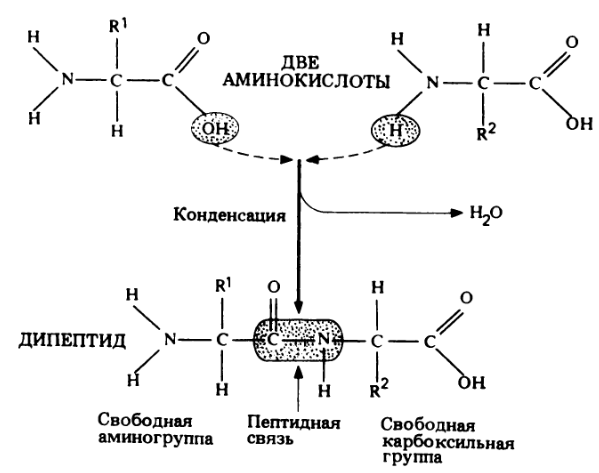
\includegraphics[width=0.5\linewidth]{pictures/dipeptid}
\caption{Схема образования пептидной связи}
\paragraph*{}Согласно Грину \cite{green_bio}
\label{dipeptid}
\end{figure}
%%%%%%%%%%%%%%%%%%%%%%%%%%%%%%%%%%%%%%%%%%%%%%%%%%%%%%%%%%%%%%%%%%%%%%%%%%%%%%%%%%%%%%%%%% 


\remember{В настоящие время в клетках растений обнаружено более 170 видов аминокислот, при этом в состав белка могут входить только 20 видов \cite{green_bio}}

\subsubsection*{Витамины: строение, классификация и функции}

\paragraph*{}\hypertarget{vitamines}{\gls{vitamines}} -- это низкомолекулярные физиологически активные органические соединения различного химического состава. В растениях синтезируются все витамины, а провитамины, которые используют затем животные для создания витаминов животного происхождения, имеют растительное происхождение (например провитамин А и витамин Д).

\paragraph*{}Витамины классифицируются на:

\begin{enumerate}

	\item водорастворимые (С, В, РР, Н, пантотеновая кислота, инозит, фолиевая кислота, пара-аминобензойная кислота),
	\item жирорастворимые (А, Д, Е, К).

\end{enumerate}

\paragraph*{}Для растений особенно важны витамины группы В,РР -- тиамин, ниацин, пиридоксин. Особенно нуждаются в притоке витаминов от фотосинтезирующих органов нефотосинтезирующие органы растения (корни, цветки, плоды).

\paragraph*{}Функция витаминов - участие в биохимических процессах в составе ферментов.

\begin{itemize}

	\item Провитамин A — \termin{каротин} (\ris \ref{vitamins}) наряду с хлорофиллом участвует в поглощении энергии света. Кроме того, он предохраняет хлорофилл от разрушения;
	\item Витамина $B_{1}$ или \termin{тиамин} (\ris \ref{vitamins}) входит в состав фермента отщепляющего углекислоту от пировиноградной кислоты и присоединяющего к этой кислоте углекислого газа;
	\item Витамин $B_{2}$ \termin{рибофлавин} (\ris \ref{vitamins}) способен соединятся с более чем 20-ю различными белками, образуя различные типы ферментов, например карбоксилазу — фермент, необходимый для превращений углеводов;
	\item Витамин C или \termin{аскорбиновая кислота} (\ris \ref{vitamins}) защищает хлорофилл от окисления. Совместно с витамином K участвует в сложных синтетических реакциях, происходящих при фотосинтезе;
	\item Витамины PP или \termin{никатиновая кислота} (\ris \ref{vitamins}), \termin{фолиевая кислота}, \termin{биотин}, \termin{пантотеновая кислота}, входя в состав ферментов, принимающих участие в процессе дыхания, в превращениях азотистых веществ, серы;

\end{itemize}

%%%%%%%%%%%%%%%%%%%%%%%%%%%%%%%%%%%%%%%%%%%%%%%%%%%%%%%%%%%%%%%%%%%%%%%%%%%%%%%%%%%%%%%%%%%%%%%%%%%%%%%%%%% 
\begin{figure}[h!]
  \centering
       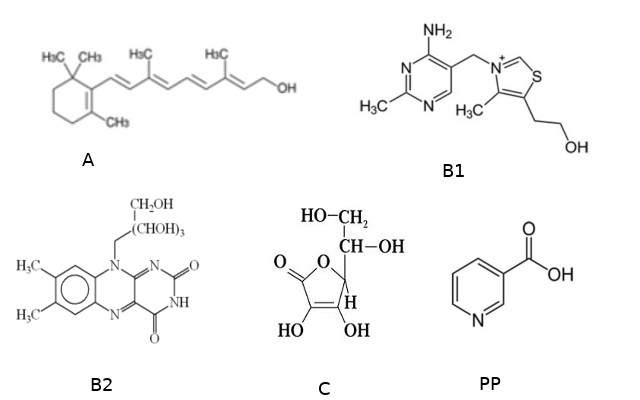
\includegraphics[width=1\linewidth]{pictures/vitamins}
\caption{Формулы некоторых витаминов}
\paragraph*{}Согласно Грину \cite{green_bio}
\label{vitamins}
\end{figure}
%%%%%%%%%%%%%%%%%%%%%%%%%%%%%%%%%%%%%%%%%%%%%%%%%%%%%%%%%%%%%%%%%%%%%%%%%%%%%%%%%%%%%%%%%%

%\subsection*{Белки и нуклеиновые кислоты}

\subsubsection*{Белки: строение, классификация и функции} 

\paragraph*{}\hypertarget{proteins}{Белки} -- это сложные биополимеры, мономером которых являются \hyperlink{aminoacids}{аминокислоты}. Доля белков в растении гораздо меньше, чем в животном организме.  

\paragraph*{}Молекула белка -- это довольно сложна, и в ее структуре можно выделить 3-4 уровня организации (\ris \ref{proteins_struct}).

%%%%%%%%%%%%%%%%%%%%%%%%%%%%%%%%%%%%%%%%%%%%%%%%%%%%%%%%%%%%%%%%%%%%%%%%%%%%%%%%%%%%%%%%%%%%%%%%%%%%%%%%%%% 
\begin{figure}[h!]
  \centering
       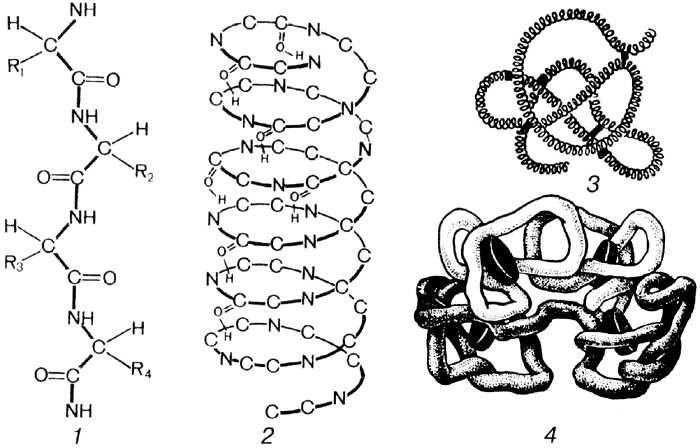
\includegraphics[width=0.7\linewidth]{pictures/proteins_struct}
\caption{Уровни организации белковой молекулы}

\label{proteins_struct}
\end{figure}
%%%%%%%%%%%%%%%%%%%%%%%%%%%%%%%%%%%%%%%%%%%%%%%%%%%%%%%%%%%%%%%%%%%%%%%%%%%%%%%%%%%%%%%%%%

\paragraph*{}При этом пространственная структура молекулы поддерживается меж- и внутримолекулярными взаимодействиями следующих типов:

\begin{enumerate}

	\item \hyperlink{pept_bound}{Пептидные связи} -- участвуют в образовании полипептидной цепочки белковой молекулы. Последовательность аминокислот в полипептидной цепочке -- это первичная структура белка.
	\item \hyperlink{question_chem_bounds}{Нековалентные водородные} связи между соседними аминокислотами -- участвуют в образовании вторичной структуры белка
	\item \hypertarget{bisulphum_bound}{Дисульфидные} связи -- образуются между остатками серособержащих аминокислот. Обуславливают формирование третичной структуры белковой молекулы
	\item Гидрофобные -- силы участвующие в формировании третичной и четвертичной структуры
	\item Электростатические -- силы участвующие в формировании третичной и четвертичной структуры. Четвертичная структура белковой молекулы присуща только сложным белкам, состоящим из нескольких белковых молекул-субъединиц. 

\end{enumerate}

%\paragraph*{}Первичная структура белковой молекулы -- это последовательность аминокислот, которая закодирована в генотипе организма. Остатки аминокислот, соединенные пептидными связями образуют полипептидную цепочку. В синтезе полипептидной цепочки принимают участие рибосомы.

%\paragraph*{}Вторичная структура белковой молекулы - это свертывание молекулы белка в пространстве за счет нековалентных водородных связей между соседними аминокислотами.

%\paragraph*{}Третичная структура белковой молекулы - это фиксирование спирали полипептидной цепочки за счет взаимодействия боковых групп аминокислот и образования гидрофобных и электростатических связей постоянной пространственной структуры. 

\paragraph*{}В основном по конфигурации белковые молекулы делят на 

\begin{enumerate}

	\item фибриллярные
	\item глобулярные

\end{enumerate}

%\paragraph*{}Четвертичная структура белковой молекулы присуща только сложным белкам, состоящим из нескольких белковых молекул. 

%\paragraph*{}Свойства белков определяются прежде всего химическими свойствами их мономеров. Белкам присуща гидрофильность (связывание с молекулами воды и образование коллоидных систем), амфотерность. 

\paragraph*{}Наиболее характерное свойство белков, присущее только им и определяемое их сложной организационной структурой (пространственной конфигурацией) -- \gls{denaturation} и обратная ей \termin{ренатурация}. 

\paragraph*{}\gls{denaturation} -- это разрушение структуры белка под действием неблагоприятных факторов, таких, как воздействие:

\begin{enumerate}

	\item температуры
	\item кислот
	\item щелочей
	\item рентгеновских или ультрафиолетовых лучей
	\item высокого давления 
	\item механического воздействия

\end{enumerate}
 
\paragraph*{}При денатурации происходит последовательное разрушение четвертичной, третичной, вторичной структуры белка. Первичная структура остается неизменной. Если воздействие фактора оказывается слабым или кратковременным, то не все уровни белка разрушаются и молекула способна к ренатурации или восстановлению третичного и четвертичного уровней организации. При воздействии фактора в течение длительного времени или в высокой концентрации денатурация белка становится необратимой. 

\paragraph*{}Классификация белков основана на их структуре. Белки делятся на протеины (простые белки) и протеиды (сложные белки).

\paragraph*{}Протеины, в свою очередь, разделяются на 7 групп. В основе данной классификации лежит способность белка растворятся в воде и его нахождение в клетки

\begin{enumerate}

\item Альбумины - растворяются в воде, находятся в \hyperlink{citoplasma}{цитоплазме}, например \termin{лейкозин} (в зародыше пшеничного зерна), \termin{легумелин} (в семянах гороха)
\item Глобулины - растворяются в слабых водных растворах солей, находятся в цитоплазме, к глобулинам относятся многие белки семян, особенно бобовых и масляничных.
\item Проламины - растворяются в 60-80\% спирте, находятся в цитоплазме, характерны исключительно для семян злаковых. Например \termin{глиадин} в семянах пшеницы и ржи, \termin{зеин} в кукурузе.
\item Глютелины - растворяются в 0,2\% щелочи, находятся в цитоплазме,
\item Фосфопротеины (казеин), содержащие фосфатный ион в составе молекулы, и не растворяются в воде, находятся в цитоплазме,
\item Протамины - находятся в ядрах клеток,
\item Гистоны - находятся в ядрах клеток и в \hyperlink{sect_rybosoms}{рибосомах}

\end{enumerate}

\paragraph*{}Протеиды представляют собой сложные белковые молекулы, состоящие из нескольких простых белков и обязательной небелковой части, которая называется простетической группой. В зависимости от состава этой группы протеиды подразделяются на 6 групп:

\begin{enumerate}

	\item нуклеопротеиды (\hyperlink{sect_rybosoms}{рибосомы}, вирусы) -- небелковая часть представлена нуклеиновой кислотой
	\item липопротеиды -- небелковая часть представлена \hyperlink{sect_lipids}{липидом}
	\item гликопротеиды -- небелковая часть представлена \hyperlink{sect_glycosids}{углеводом}
	\item фосфопротеиды -- в качестве небелковой части выступает остаток фосфорной кислоты
	\item гемопротеиды -- в качестве небелковой части выступает железо связанное с порфириновым кольцом
	\item металлопротеиды -- в качестве небелковой части выступает ион металла

\end{enumerate}

\paragraph{Функции белков}

\begin{enumerate}

	\item ферментативная (т.е. ведут катализ биохимических реакций),
	\item структурная (строительные молекулы),
	\item запасные вещества
	\item транспортная (перенос кислорода, углекислого газа, жиров, железа и т.д.),
	\item сократительная,
	\item защитная (токсины)
	\item Управляющая (гормоны).

\end{enumerate}

\subsubsection*{Ферменты}

\note{По своей природе ферменты являются белками, играющими, однако ключевую роль в функционировании живых систем}

\paragraph*{}\hypertarget{enzimes}{Ферменты} (энзимы) — биологические \hyperlink{catalith}{катализаторы} белковой природы.
%Катализатор — вещество, увеличивающее скорость химической реакции, но само при этом не расходующиеся. Как и белки, ферменты обладают первичной, вторичной, третичной и четвертичной структурой.
\paragraph*{}В зависимости от особенностей структуры молекулы, ферменты делятся на:

\begin{enumerate}
\item Однокомпонентные -- молекула состоит только из белка
\item Двухкомпонентные -- в состав молекулы фермента, кроме самого белка, входит небелковый компонент. 

\end{enumerate}

\paragraph*{}В том случае, если небелковый компонент прочно связан с белком, он носит название \termin{простетическая группа}. Если же небелковый компонент может отсоединятся от белка, он называется \termin{коферментом}. В качестве коферментов могут выступать различные ионы ($Fe^{2+}$, $Cu^{2+}$). 

\remember{Белковая часть сложного фермента — апофермент специфичен для каждого вида растений, а коферменты, для типа реакции}

%\paragraph*{}В состав двукомпонентных ферментов входит кроме самого белка небелковый компонент, который может быть либо прочно связан с белком — простетическая группа, либо слабо связан — кофермент. В качестве коферментов могут выступать различные ионы (Fe ++, Cu ++). Белковая часть сложного фермента — апофермент специфичен для каждого вида растений, а коферменты, для типа реакции. 

%\paragraph*{}Локализация ферментов. Чаще всего ферменты находятся внутри клетки или отдельных ее органеллах: белки цитохромы в митохондриях. Кроме того существуют экзоферменты — ферменты, находящиеся на оболочках клеток (чаще всего корня).

%\textbf{Механизм ферментного катализа}

%\paragraph*{}Все реакции в клетке проходят в водной среде. Для реакции молекула должна обладать энергией активации. Фермент снижает энергию активации. Теория ключ — замок. 

\paragraph*{}Катализ химической реакции ферментом осуществляется в результате образования фермент-субстратного комплекса. В результате происходит 

\begin{itemize}

\item либо сближение реагирующих молекул 
\item либо создание напряженных химических связей путем их растягивания

\end{itemize}

\note{Субстрат должен соответствовать активному центру не только пространственно, но и по распределению зарядов, расположению групп атомов и так далее. Обычно для описания взаимодействия молекул фермента и субстрата используют образ ключа и замка. То есть форма молекулы субстрата подходит к форме активного центра фермента как ключ подходит к определенному замку. Однако, в отличии от ключа и замка, при взаимодействии изменяется форма молекул как субстрата, так и фермента. То есть происходят конформные изменения фермента и субстрата.}

\paragraph*{}Продукты реакции отделяются от фермента и молекулы фермента регенерируются. 

\remember{Благодаря своей способности регенерироваться, то есть возвращаться к первоначальному состоянию, одна и та же молекула фермента может катализировать большой объем превращений}

\paragraph*{}Свойства ферментов

\begin{enumerate}

	\item Высокая спцифичность. Реакция — фермент, Тип реакции — фермент. (Неоганические катализаторы неспецифичны.)
	\item Обратимость действия фермента.

\end{enumerate}

\paragraph*{}Факторы, влияющие на активность фермента.

\begin{enumerate}

	\item Температура. Оптимум для ферментов 20-30~ \celsius. Пессимум — 70-80~ \celsius градусов. Скорость ферментного катализа, как и других химических реакций подчиняется правилу ВанГоффа.
	\item Кислотность среды — для разных ферментов нужны разные значения кислотности среды: инвертаза — 4,7, фосфатаза — 5.
	\item Наличие активаторов и ингибиторов. Актиавторами чаще служат ионы щелочных металлов — K, Ca, Na, а ингибиторами — ионы тяжелых металлов, вызывающие денатурацию белка. Кроме того существуют спецефические ингибиторы.

\end{enumerate}

\paragraph{Регуляция ферментативной активности}

\paragraph*{}В настоящие время известны следующие механизмы внутриклеточной регуляции активности ферментов:

\begin{enumerate}

	\item Метаболитная регуляция. Происходит в результате изменения концентрации метаболитов и не затрагивает активность или число ферментных молекул.

	\item Ферментная регуляция. При этом типе регуляции изменяется активность ферментов. Изменение ферментативной активности может осуществляться несколькими путями: 
	\begin{itemize}
		\item Обратимое или необратимое превращение неактивных предшественников ферментов в активные ферменты. \note{Например, b-амилаза в клетках эндосперма семян злаковых находится в инактивированом состоянии из-за соединения с запасными белками посредством \hyperlink{bisulphum_bound}{дисульфидных} связей ( -S-S-). К началу прорастания семян из живых клеток алейронового слоя в эндосперм поступают вещества, разрушающие дисульфидные связи. Активированная b-амилаза принимает участие в гидролизе запасного крахмала}
		\item Изменение активности фермента под влиянием веществ \termin{эффекторов}. Связываясь с ферментом, эффекторы могут либо повышать его активность (\termin{активаторы}) либо уменьшать ее (\termin{ингибиторы}). Эффектор может влиять на активность фермента, взаимодействуя с активным центром (\termin{изостерический эффект}) или изменяя конформацию ферментной молекулы в результате связывания с ее дополнительным управляющим (аллостерическим) центром (\termin{аллостерический эффект}). Изостерический эффект происходит в том случае, когда эффектор и субстрат похожи по своему строению и конкурируют друг с другом за активный центр фермента. Такой тип ингибирования называют конкурентным ингибированием.
	\end{itemize}

	\item Генная регуляция. Количество ферментных молекул в клетке изменяется из-за включения или выключения синтеза ферментов. Регулирующие факторы действуют на \gls{dna}, \gls{rna} или \hyperlink{sect_rybosoms}{рибосомы}.

	\item Мембранная регуляция. Различают контактную и дистанционную мембранную регуляцию активности ферментов. Контактная регуляция – связывание ферментов с мембранами или их освобождение меняет их активность. Дистанционная мембранная регуляция активности ферментов осуществляется косвенным путем в результате транспорта через мембраны субстратов и коферментов, удаления продуктов реакции, ионных и рН сдвигов в компартментах клетки.
\end{enumerate}

%\paragraph*{}Ферменты, имеющие основной и аллостерические активные центры, называют аллостерическими. Аллостерический фермент характеризуется тем, что его активация происходит не за счет активного центра, а за счет присоединения активатора или ингибитора к другому участку молекулы фермента, где при этом образуется аллостерический активный центр. 

%\paragraph*{}В отличие от обычных активаторов и ингибиторов основных активных центров, активаторы и ингибиторы аллостерических центров называются эффекторами.

\paragraph{Классификация ферментов} 

\paragraph*{}В данное время общепринята международная классификация ферментов, согласно которой все ферменты разделяются на шесть классов. При этом название ферментов образуется, как правило, от названия субстрата, на который действует данный фермент или от названия катализируемой ферментом реакции. Название фермента заканчивается на суффикс \tcbox{-аза}\hfill

\begin{enumerate}

\item \termin{Оксидоредуктазы} -- ферменты, катализирующие окислительно-восстановительные реакции. Чаще окисление происходит путем переноса водорода и электронов по следующей схеме: $AH_{2} + B = A + BH_{2}$ 


\item \termin{Трансферазы} -- ферменты переносящие радикалы между молекулами по схеме AX + B = BX + A. Среди трансфераз выделяют 
	
	\begin{itemize}
	
	\item \termin{Протеазы} -- ферменты расщепляющие белки \termin{папаин} \footnote{Папаин расщепляет и белки, и жиры, и углеводы}. 
	\item \termin{Карбогидразы} -- ферменты синтеза и расщепления углеводов, 
	\item \termin{Эстеразы} -- ферменты синтеза и расщепления сложных эфиров,
	\item \termin{Амидазы} -- ферменты синтеза и расщепления нуклеотидов и азотистых оснований.

	\end{itemize}

\item \termin{Фосфотрансферазы} -- это ферменты, катализирующие перенос остатка фосфорной кислоты. В результате действия фосфотрансфераз образуются фосфорные эфиры различных органических соединений, многие из которых обладают повышенной реакционной способностью и более легко вступают в последующие реакции. \note{Следовательно, фосфорилирование органических соединений можно считать процессом их активации. Чаще всего донором фосфатных групп является молекула аденозинтрифосфорной кислоты (\gls{atp}).} Фосфотрансферазы, использующие в качестве донора фосфатной группы молекулу \gls{atp}, называются \termin{киназами}. К киназам относится, например, глицеролкиназа, ускоряющая перенос остатка фосфорной кислоты от молекулы \gls{atp} к молекуле глицерина: 
 

\item \termin{Изомеразы} -- ферменты катализирующие превращение одних веществ в другие. Например трифосфат-изомераза в процессе брожения превращает 3-фосфоглицериновый альдегид в  фосфидоксиацетон

\item \termin{Лиазы} -- ферменты ращепляющие веществ без использования воды по схеме AB = A + B

\item \termin{Лигазы} -- ферменты, принимающие участие в синтезе веществ. Например ДНК-лигазы катализируют образование фосфодиэфирной связи в однонитевом разрыве (ОР) ДНК между смежными 3’-гидроксильным и 5’-фосфатным концами разорванной нити. 

\item \termin{Гидролазы} -- ферменты, принимающие участие в расщеплении сложных веществ с участием воды, например фермент, гидролизирующий гликозид \termin{синигрин}, содержащийся в горчичном семени

\end{enumerate}

%\paragraph*{}Нуклеиновые кислоты дать на самостоятельное изучение

\subsection*{Вопросы и задания для самоконтроля}

\begin{enumerate}
	\item Самостоятельно по учебнику химии или физиологии растений повторите строение молекулы \hypertarget{question_aqua}{воды} например по учебнику химии Н.Е. Кузьменко \cite{chem_kuzmenko_eremin}. Благодаря каким особенностям структуры молекулы вода имеет харктерные для нее свойства?
	\item \hypertarget{question_vakual_rep}{Повторите} ранее изученный материал о строении клетки и опишите строение и функции \hyperlink{cell_vakuol}{центральной вакуоли}.
	\item Повторите строение молекулы и химические свойства углеводов. Что такое \hypertarget{question_isomeria_gluc}{изомерия}, какие типы изомерии свойственны углеводам?
	\item Какой, \hypertarget{question_lipid}{жир} по вашему мнению будет жидких -- тристеорин или триолеин?\cite{green_bio}
	\item По учебнику химии, например Н.Е. Кузьменко \cite{chem_kuzmenko_eremin}, повторите особенности строения и химических свойств \hypertarget{aminoacids}{аминокислот}. Приведите несколько примеров химических реакций, подтверждающих амфотерные свойства аминокислот.
	\item Что такое \hypertarget{catalith}{катализатор}? Какова связь между веществом катализатором и энергией активации катализируемой реакции? 
	\item По учебнику химии повторите тему <<\hypertarget{question_chem_bounds}{Химическая связь}>>. Каковы механизмы образования химической связи ковалентного и водородного типов?
\end{enumerate}